\subsection{ADO.NET Entity Framework}
\label{sub:adonet}
The ADO.NET is designed by Microsoft with the purpose of making a disconnected database architecture to use with the .NET framework \cite{adonetDesignGoal}.

The ADO.NET EF is an object relational mapping framework \cite{adonetEntityFramework}.

Together with the ADO.NET Entity Data Model Designer and a SQL Server ADO.NET EF gives a strong tool for mapping a database and using the data in a object oriented matter, without dealing with the transformation from entity to class and from tuple to object. 
The Designer is built into Visual Studio Ultimate. 

Using the ADO.NET and the Entity Data Model Designer can be done in two ways. 
The  model can be created from an already existing database or by creating the model and generate a database from this \cite{adonetEntityDataModelDesigner}.
We use the last approach and creates the database from the model. 
In this way we do not have to worry about setting the right foreign keys and relational tables. Instead we get a fully functional model linked to a database. 

Our model as it is in the ADO.NET Entity Model Designer is shown on figure \ref{}
\begin{figure}
	\centering
		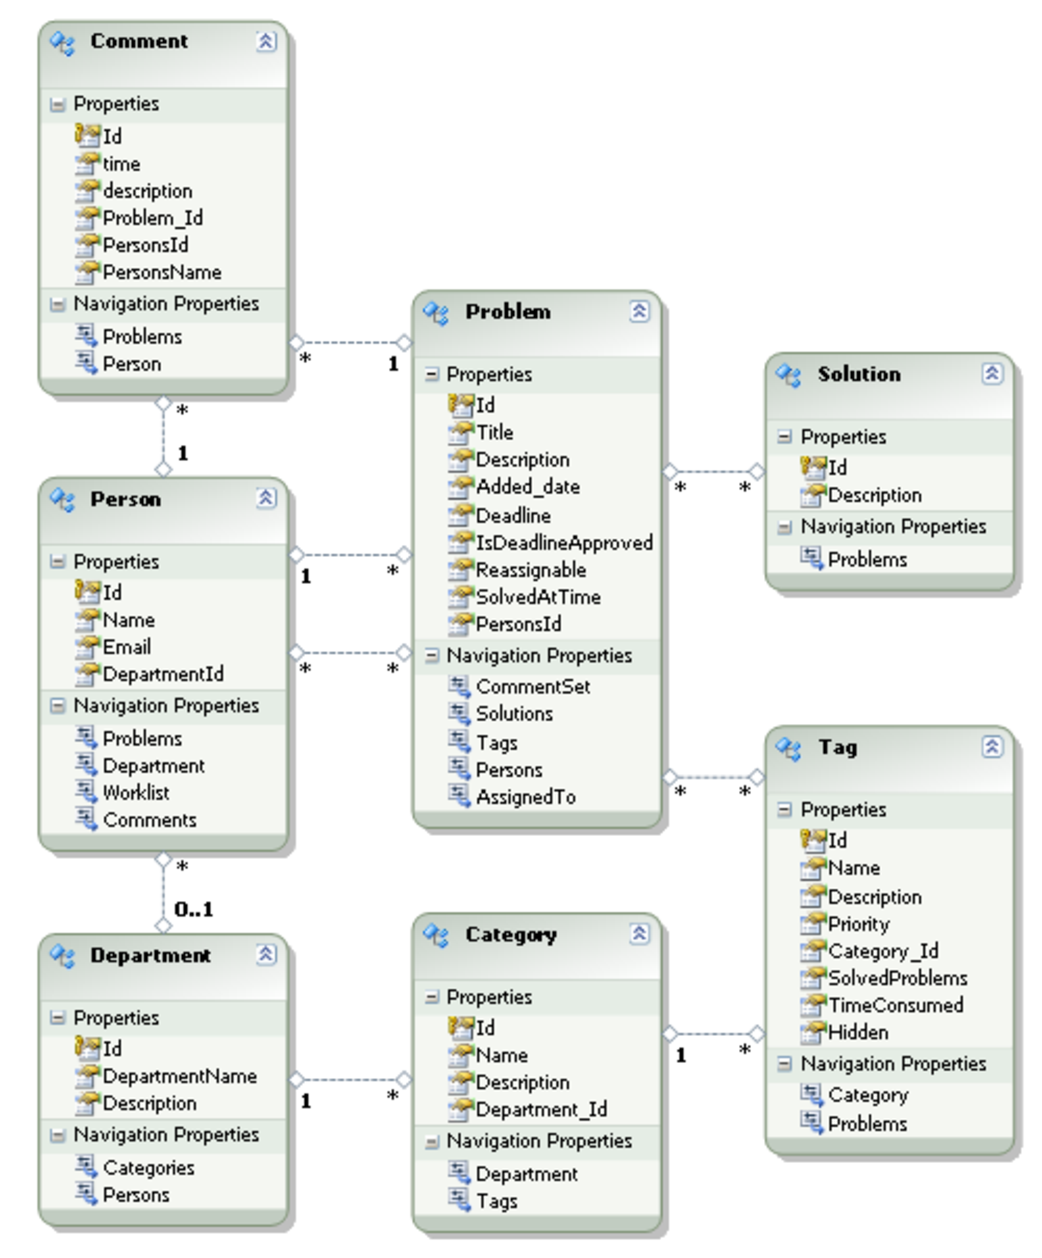
\includegraphics[scale=0.8]{input/implementation/mvc/Model.pdf}
	\morscaption{Our model as it is seen in the ADO.NET Entity Data Model Designer.}
	\label{fig:balanceWorkloadDiagram}
\end{figure}






 % Cite 
 % adonetDesignGoal - http://msdn.microsoft.com/en-us/library/7b13c12s(v=VS.71).aspx 
 
 % adonetEntityFramework - http://msdn.microsoft.com/en-us/library/aa697427(VS.80).aspx
 
 % adonetEntityDataModelDesigner - http://msdn.microsoft.com/en-us/library/cc716685.aspx
 
 % adonetGeneral - http://msdn.microsoft.com/en-us/library/h43ks021(VS.71).aspx